\documentclass{minimal}
\usepackage{tikz}
\usetikzlibrary{patterns}

\begin{document}

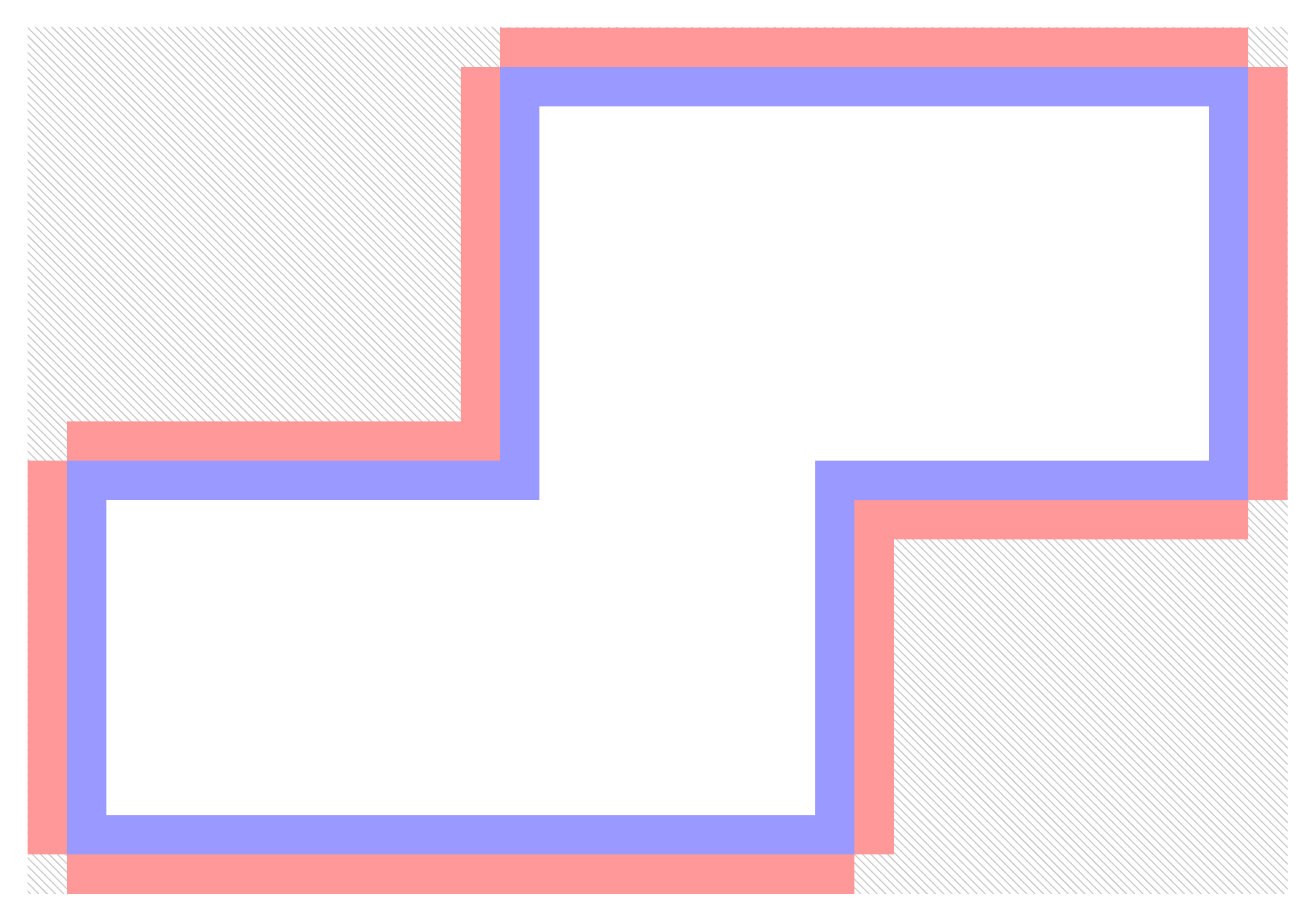
\begin{tikzpicture}[auto, scale=.5]
    \fill [pattern=north west lines, pattern color=gray!40] (-1, -1) rectangle (31, 21);
    \fill [red!40] (-1, 0) -- (-1, 10) -- (0, 10) -- (0, 11) -- (10, 11) -- (10, 20) -- (11, 20) -- (11, 21) --
                    (30, 21) -- (30, 20) -- (31, 20) -- (31, 9) -- (30, 9) -- (30, 8) -- (21, 8) -- (21, 0) -- (20, 0) -- (20, -1) --
                (0, -1) -- (0, 0) -- cycle;
    \fill [blue!40] (0, 0) -- (20, 0) -- (20, 9) -- (30, 9) -- (30, 20) -- (11, 20) -- (11, 10) -- (0, 10) -- cycle;
    \fill [white] (1, 1) -- (19, 1) -- (19, 10) -- (29, 10) -- (29, 19) -- (12, 19) -- (12, 9) -- (1, 9) -- cycle;

\end{tikzpicture}

\end{document}
